\chapter{Performance Evaluation}
In machine learning una delle fasi più importanti è la valutazione del modello,
utile per capire la sua bontà e per avere delle metodologie di confronto con gli
altri.

Innanzitutto per valutare il modello non si considerano gli errori, calcolati come
scarto, delle predizioni sui dati di training. Questo perché successivamente si 
otterranno nuovi dati completamente differenti da quelli utilizzati per la fase
di training, invalidando la metrica calcolata.

La valutazione del modello permette fin da subito di rilevare eventuali comportamenti
di underfitting o di overfitting. Queste dinamiche vengono illustrate nella figura 
\ref{fig:overfitting-vs-underfitting}, in cui si può notare che un modello all'aumentare
della sua complessità si avrà tre fasi:
\begin{itemize}
    \item \textbf{fase di underfitting}: fase in cui il modello è ancora semplice
    per cui gli errori sul training e sul test sono elevati. Questo significa che
    si è in underfitting perché il modello non fitta bene sul training e, in aggiunta,
    non riesce a generalizzare.
    \item \textbf{fase ideale}: fase in cui il modello ha una complessità adeguata
    per cui non è troppo semplice da andare in underfitting e non è troppo complesso
    da andare in overfitting. Questa fase è ideale perché si ha un buon fit sul training
    e una buona generalizzazione sul test set
    \item \textbf{fase di overfitting}: fase in cui il modello è troppo complesso
    quindi si fitta molto bene sul training ma non riesce a generalizzare sul test.
    Questo comporta errori molto piccoli sul training, con un conseguente aumento
    degli errori sul test.
\end{itemize}

\begin{figure}[!ht]
    \centering
    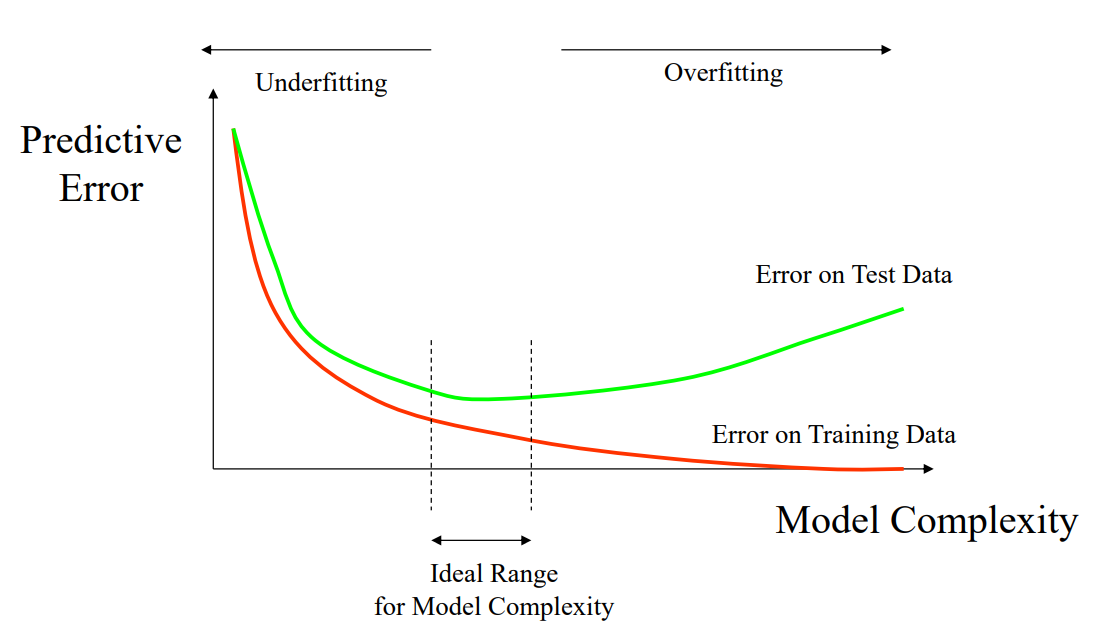
\includegraphics[width=0.7\textwidth]{img/performance evaluation/overfitting_vs_underfitting.png}
    \caption{Rappresentazione dell'overfitting e underfitting}
    \label{fig:overfitting-vs-underfitting}
\end{figure}

Le metriche di valutazione evidenziano tre componenti:
\begin{itemize}
    \item bontà del modello sul train
    \item bontà del modello sul test
    \item complessità del modello (quanti parametri): spazio, tempo in termini di $O$
\end{itemize}

Per le metriche sarà fondamentale introdurre la \textbf{matrice di confusione}, in cui 
\begin{equation}
    T[i,j] = \# \ \text{degli esempi etichettati come} \ i \ \text{predetti come classe} \ j
\end{equation}
Se si è nel caso di classificazione binaria allora:
\begin{itemize}
    \item $i=0, j=0$, true positive, \textbf{TP}: esempi positivi predetti come positivi
    \item $i=0, j=1$, false negative, \textbf{FN}: esempi positivi predetti come negativi
    \item $j=1, j=0$, false positive, \textbf{FP}: esempi negativi predetti come positivi
    \item $j=1, j=1$, true negative, \textbf{TN}: esempi negativi predetti come negativi 
\end{itemize}
L'obiettivo sarà quello di massimizzare la diagonale e minimizzare il resto.
\section{Metriche di valutazione}
Le metriche di valutazione sono differenti e si possono calcolare in modo aggregato
su tutte le classi oppure si possono calcolare su una classe alla volta e in un 
secondo momento aggregarle secondo delle medie.

Le metriche aggregate sono:
\begin{itemize}
    \item \textbf{Tasso di errore}:
    Metrica più naturale che consiste nel calcolo della proporzione degli errori su 
    tutto l'insieme di istanze dato in input al modello. Gli errori possono essere 
    calcolati secondo lo scarto o secondo le distanze.
    \item \textbf{Accuracy}:
    Misura la proporzione di istanze correttamente classificate su tutto l'insieme
    dato in input sul set.
    \begin{equation}
        Ac = \frac{TP+TN}{TP+TN+FP+FN}
    \end{equation}
    \item \textbf{Precision}:
    La precision misura la proporzione di esempi positivi predetti come positivi (TP)
    sul numero totale di esempi predetti come positivi.
    \begin{equation}
        P=\frac{TP}{TP+FP}
    \end{equation}
    \item \textbf{Recall}:
    La recal misura la proporzione di esempi positivi predetti come positivi (TP) sul
    numero totale di esempi positivi predetti come positivi ed esempi positivi predetti
    come negativi.
    \begin{equation}
        R=\frac{TP}{TP+FN}
    \end{equation}
    \item \textbf{F-measure}:
    La F-measure calcola la media armonica della precision e della recall.
    \begin{equation}
        \frac{2\cdot P\cdot R}{P+R}
    \end{equation}
\end{itemize}

Le ultime tre le calcoleremo sulle singole classi:
\begin{itemize}
    \item 
\end{itemize}


Queste misurare non le useremo sulle classi aggregate ma sulle singole classi
Se 3 classi allora abbiamo 3 misure di precision, recall, f-measure


PEr aggregare queste misurare useremo:
\begin{itemize}
    \item macro avg: fa la media tra le diverse classi delle singole metriche 
    (classi con uguale importanza)
    \item micro avg: media pesata della performance rispetto alla cardianlità 
    della classe (classe con diversa importanza) (possiamo specificare un peso 
    a piacere l'importante che si garantisca il range della metrica)
\end{itemize}


Per confrontare i modelli si utilzizano le curve ROC e mettono a confronto TP rate
e FP rate. La curva ROC non sono altro che la valutazione del modello con diverse
soglie decisionali del modello da 0 a 1, EX: Bayes si sceglie al posto di 0.5 a 0.8 
Più la soglia tende a 1 allora si ha un modello conservativo miglioreremo la precision
peggiorando la recall
Più abbassiamo la soglia si aumenta la recall ma si abbassa la precision.
La ROC si costruisce eseguendo i modelli con treshold diverse e si ricalcola la 
matrice di confusione diversa e quindi TPR e FPR differenti.

Nel confronto tra modelli avremo una curva per ogni modello e questo permette di 
studiare il suo comportamento. Generalmente si confronta il singolo modello con il
classificatore perfetto (verde) e quello randomico (rosso). Il modello migliore è
il dominante. Quando le linee si intersecano allora si deve studiare l'area sottesa 
all'area AUC (scalare). Quindi prendo quello con AUC maggiore. Può essere utilizzato 
in trainig e testing.
Hanno delle limitazioni:
- AUC sono inutili quando le classi hanno diversa importanza 
- sensibile allo sbilanciamento perché una classe sarà più pesante sui risultati


Curve di apprendimento sono delle curve che possiamo disegnare che dicono al variare
della numerosità del campione come si comporta il modello in termini di accuratezza.
Le barre blu rappresentano la varianza della predizione. I punti rappresentano
le media della metrica scelta delle singole esecuzioni del metodo eseguiti su tutte le combinazioni
di 5 cambino di training. 
Quanti dati sono necessari per avere un modello con performance accettabile in termini
di tempo di apprendimento e della performance. Molto pesante ma spesso si costruisce 
parzialmente.

Prob grande => 10000 istanze 
Più grande il campione allora si effettuerà una suddivisione train test 80 20

Se il modello deve essere messo in produzione allora effettuo il training su tutto 
dataset.

I dati di test non devono essere usati per il tuning degli iperparametri. GLi
iperparametri possono essere i k cluster o anche le soglie del modello e si trovano
sul validation.

Per dataset piccoli si esegue train test più volte in crossvalidation.

Per la generazione degli insiemi per crossvalidation spesso chiedono la stratificazione
ovvero se ho una classe popolosa allora questa deve essere uguale sia in training sia in
test. Si deve sempre stratificare (generalmente si usa k=10 fold). 

Quando abbiamo dataset estremamente piccoli <100 istanze e quindi si usa la tecninca
di leave-one-out. Crossvalidation di 1 test e tutto il resto training

\section{Affidabilità delle misure di performance}
Ogni iterazione della k-fold mi da una misura di performance, posso calcolare la media
tra tutte le performance. Non si può utilizzare la media per confrontare perché 
perdiamo la variabilità. Quello che si fa è stimare gli intervalli di confidenza
perché:
\begin{itemize}
    \item si capisce la posizione della media
    \item ci da la robustezza  (ampiezza intervallo di confidenza) meglio quello
\end{itemize}
2 modelli

stessa media , il primo IC 0.7,0.8 mentre il secondo 0.5 e 1, il migliore è quello
col più piccolo intervallo. Se gli intervalli non si sovrappongono e hanno la 
stessa ampiezza è la situazione migliore.

Altro approccio di confronto tra modelli si usa il test di significatività 
- test paired quando entrambi i modelli hanno imparato nello stesso modo sugli stessi dati
- test unpaird altrimenti

Non guardare solo la performance numerica
Considera sempre la complessità